% Chapter Template

\chapter{Implementation} % Main chapter title

\label{implementation} % Change X to a consecutive number; for referencing this chapter elsewhere, use \ref{ChapterX}

\section{Technology stack}
\label{technology}
The main library that was used is \textit{scikit-learn} \cite{scikit-learn}. \textit{Scikit-learn} is a robust machine learning library for Python. It is build upon NumPy, SciPy, and matplotlib. It is also open source and commercially usable with the BSD license. There is a lot of documentation available for \textit{scikit-learn}. This library was chosen since the library offers the most important algorithms, the documentation. The programming language, Python, is also good for prototyping.  \\
\\
Most algorithms that have been explained in Section~\ref{algorithms} are implemented in \textit{scikit-learn}. The stable version of this library does not implement neural networks. However, the unstable version does include neural networks. \\
\\
\textit{Scikit-learn} also contains different methods to visualise machine learning algorithms such as a graph to show the learning curve. These can be a useful tool to evaluate the performance of machine learning algorithms. It also contains methods to calculate the F-score. This is useful since that means that mistakes when calculating the F-score are less likely to happen.

\subsection{Program execution}
The implementation works in different steps. A JSON config file is used to define the elements that are used within the program. This contains the data to be used for learning, for checking, the machine learning algorithm, etc. A full explanation of the config file as well as a general user guide can be found in Appendix~\ref{config}. \\
\\
Once the config file has been read, the program can start the training phase. In this phase the specified algorithm is used and trained using the given data. Afterwards the prediction phase starts.  This phase uses the prediction data and gathers all results. The structure of the program and the modules reflect these different phases.

\subsection{Structure}
\label{modules}
The implementation is build to be modular. New components can easily be added. Details on how to add new components to these modules is explained in the developer guide in Appendix~\ref{framework}. The first module is the machine learning module. This module contains all machine learning algorithms that can be used. \\
\\
There is also a feature module. This module contains the available classes that can be used to extract features from the flows. A loader module contains all classes required to load the data from the different datasets. \\
\\
A training module contains the different classes used for training. These classes use a loader class and pass the data to the machine learning algorithm. They define which data is supposed to be used (for example, using only abnormal behaviour and leaving out the normal behaviour). \\
\\
Finally there is a results module. This module receives all the output from the machine learning algorithms and has to log these or visualise them.

\section{Datasets}
\label{datasets}
In order to test the implementation and the algorithms, different datasets were used. Each dataset is used to test a different aspect of the machine learning algorithms. First, a subset of a dataset has to be chosen to be fed to the machine learning algorithms for learning. Afterwards, using the method seen in Section~\ref{evaluationHypothesis}, the algorithm is tested using another subset of the same dataset. \\\\
In the third step, the algorithms are tested using real-world data that is labeled. Finally, in the fourth step, the algorithms are tested using raw, unlabeled real-world data. This is to make sure that the algorithm performs well on unprocessed real-world data. Several datasets have been used to test the machine learning algorithms.

\subsection{CTU-13 Dataset}
The CTU-13 dataset has been used for steps one to three for the testing of the machine learning algorithms. This is a labeled dataset. It contains botnet behaviour, normal and background traffic. The data was captured in the CTU University, Czech Republic, in 2011. It consists of thirteen different captures, each of which run a different botnet malware. Figure~\ref{fig:ctu13-2} shows the amount of data within each capture. Note that the captured data is only from a couple hours. The flows within the dataset contain extra information. Each flow also contains the TCP flags obtained by OR-ing the TCP flags field of all packets of the flow. \cite{garcia2014empirical} 

 \begin{figure}[H]
\centering
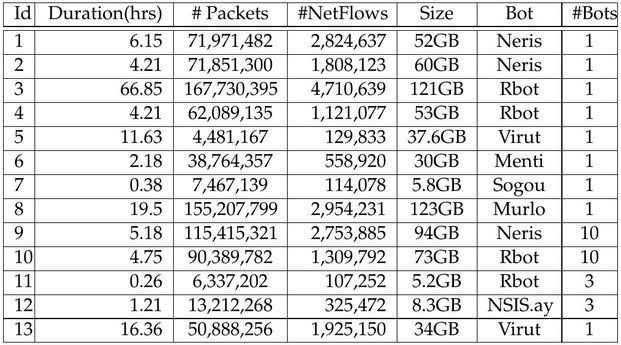
\includegraphics[width=1\textwidth]{Figures/ctu13-2}
\decoRule
\caption[Amount of data and botnet type for each capture]{Amount of data and botnet type for each capture. \cite{garcia2014empirical}}
\label{fig:ctu13-2}
\end{figure}

\noindent Each capture contains only a small amount of botnet samples as seen in Figure~\ref{fig:ctu13-1}.  Most flows are background flows. This is expected of botnet behaviour since it does not generate an large amount of network traffic. The actual labeling is much more detailed as compared to Figure~\ref{fig:ctu13-1}. Each flow is labeled with its exact source. This could be google analytics, google webmail or a windows update. The flows within the dataset only contain the regular information that is found within netflow. The abnormal behaviour within this dataset is internal abnormal behaviour. In the evaluation chapter, this dataset is called the CTU dataset.

 \begin{figure}[H]
\centering
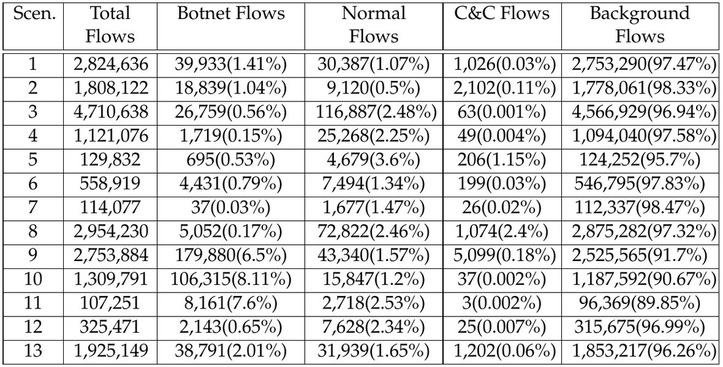
\includegraphics[width=1\textwidth]{Figures/ctu13-1}
\decoRule
\caption[Distribution of labels in CTU 13 Dataset]{Distribution of labels in CTU 13 Dataset. \cite{garcia2014empirical}}
\label{fig:ctu13-1}
\end{figure}

\noindent It is also important to note that each capture contains different botnet behaviour. In Figure~\ref{fig:ctu13-3}, the characteristics of the different botnet captures are shown. During experiments, it is important that the machine learning algorithm is trained and tested using data with the same characteristics. This is because each characteristic exhibits unique behaviour. The labeling of the flows is also different between the different captures. This makes it difficult to train with one capture and test with another capture. Even among the captures with the same botnet characteristics, there is different labeling between the captures. For this reason, it was chosen that the algorithm would be trained and tested using a single capture. The capture itself is chosen at random. This is done to make sure that experiments were done across different captures. Using every capture would explode the training set and make testing unpractical.

 \begin{figure}[H]
\centering
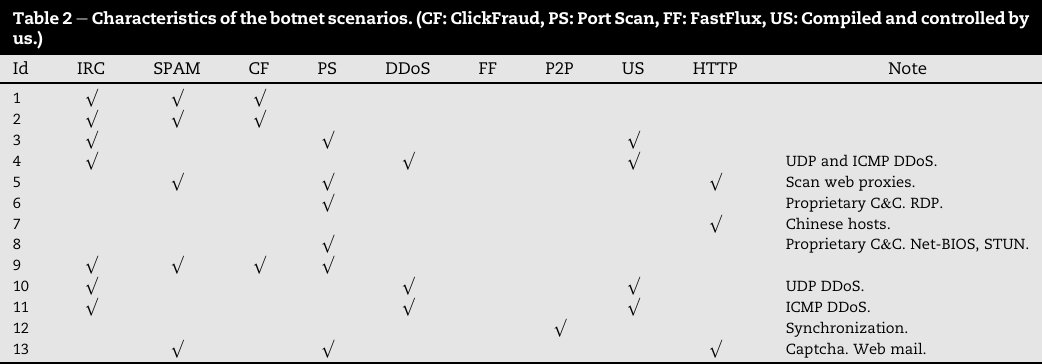
\includegraphics[width=1\textwidth]{Figures/ctu13-3}
\decoRule
\caption[Characteristics of botnet scenarios]{Characteristics of botnet captures. \cite{garcia2014empirical}}
\label{fig:ctu13-3}
\end{figure}

\subsection{Tracelabel Dataset}
This dataset has been used for steps one to three for the testing of the machine learning algorithms. The tracelabel dataset is a database constructed at the University of Twente in September 2008. It contains flow data of traffic collected from a honeypot that was positioned in the network of the university. The honeypot ran sevaral network services such as ftp, ssh, http, etc. The honeypot only captured abnormal behaviour. As such, all of the data within the dataset is actual abnormal behaviour. \cite{sperottoIPOM2009} \\
\\
The flows within the dataset contain extra information. Each flow also contains the TCP flags obtained by OR-ing the TCP flags field of all packets of the flow.  In Table~\ref{tab:tracelabel}, the labeling that is used within this dataset can be seen. The abnormal behaviour within this dataset is external abnormal behaviour. In the evaluation chapter, this dataset is called the SQL dataset.

\begin{table}[H]
\caption{Labeling of the Tracelabel dataset.}
\label{tab:tracelabel}
\centering
\begin{tabular}{l c r}
\toprule
\tabhead{Id} & \tabhead{label} & \tabhead{Explanation}\\
\midrule
 1 & ssh\_scan & An ssh scan \\
 2 & ssh\_conn & Unauthorized ssh connection attempt \\
 3 & ftp\_scan & An ftp scan \\
 4 & ftp\_conn & Unauthorized ftp connection attempt \\
 5 & http\_scan & An http scan \\
 6 & http\_conn & Unauthorized http connection attempt \\
 7 & authident\_sideeffect  & Unauthorized identification attempt \\
 8 & irc\_sideeffect  & Suspicious irc traffic \\
 9 & icmp\_sideeffect & Suspicious icmp traffic \\
\bottomrule
\end{tabular}
\end{table}

\subsection{EDM Dataset}
This is a dataset of unlabeled netflow data gathered from the EDM network. The EDM or the Expertise centre for Digital Media, which is located at the science park at UHasselt. The EDM is the ICT research institute of Hasselt University and has around $47$ researchers working there. The dataset is gathered from the entire EDM network. The flows are gathered at the edge of the network and contain both incoming and outgoing flows. \\
\\
This dataset has been used for step four for the testing of the machine learning algorithms, to check if the machine learning algorithms perform well on unprocessed real-world data. It spans from the 18th of Februari, 2016 till the 24th of March  2016. The data spans from 10am till midnight. This dataset is used mainly to check whether the machine learning algorithms perform well on real-world data.

\subsection{Cegeka Dataset}
A dataset from Cegeka has been used. Cegeka is a full-service ICT-business with offices in Belgium, the Netherlands, Poland and Romania. Cegeka has three datacenters which are all located in Belgium. They are located in Hasselt, Leuven and Veenendaal. The dataset contains network data from the datacenter in Hasselt. \\
\\
The dataset spans three days, from the third of April till the  fifth of April. This dataset contains unlabeled netflow data. It also contains logs from firewalls. These logs can be used to check whether the machine learning algorithm has a good performance. 

\section{Feature selection}
\label{featureSelection}
A lot of information can be found within a flow as explained in Section~\ref{flow}. The standard attributes of a flow have been chosen to be used as features. The extra information such as the TCP flags that are set have not been used in every step of the evaluation process since they are not available in all of the datasets that have been used. However, they have been used in some experiments to test their effects using the datasets that do have this information. \\
\\
In the implementation, the features are all seen as continuous data. In order to use discrete data, a conversion has to be made to allow them to be used as continuous data. Both source and destination IP addresses are used as features. They were used as contiguous data by using the IP address in decimal format. Different features have been used for IP addresses and MAC addresses. \\
\\
Another option was to look at IP addresses as if they were discrete features. For example, it could be possible to only look at the three least significant bytes of the IP address. This is a simple method to divide IP addresses into "subnets". However, this is not exactly a correct subnet. The best method would be to use the longest prefix matching to find the subnet to which an IP address belongs. However, it is difficult to find this information. Another method would be to use something like the country of origin. Using an API to find out the country of origin of an IP could be used to make a discrete feature. This divides IP addresses in different regions similar to a subnet which makes it a good subsitute for longest prefix matching.\\
\\
The source and destination ports are also used as features. Ports are not continuous information. The difference between using port $21$ and port $22$ is just as big as the difference between using port $22$ and $1024$. This means that ports are discrete data. One method to solve this is to make a different feature for each port. The possible values for each feature would be $1$ or $0$. However, this has as effect that there are a lot of features, in the tens of thousands. This is very inefficient and impractical. The solution that has been chosen in to make a feature that determines whether the port is one of the $1024$ well known ports or another port. \\
\\
These protocols are all IP protocols. Protocols which are encapsulated within an IP header. They mainly belong to the transport layer, but can also contain network layer protocols such as ICMP. Protocols are also discrete data. However, there are not that many different protocols. This means that it is viable to use a different boolean feature for each protocol. \\
\\
The amount of packets and the amount of bytes in the flow are both continuous by nature. They can just be used as continuous features. The duration is also continuous and is represented as such.\\
\\
The ability to remove this limitation is behind a paywall. The starting time of a flow has not been used. Manipulations of the starting time as described in Section~\ref{timeflow} has not been used since there is not enough data for it to be useful. There is only training data from a timeframe of a couple hours. Different data sets were used for the training and the starting time of the flows do not match between these data sets. This means that, since the starting time is not consistent, results from this is also not consistent or representative. However, such a feature does seem promising if the training data is consistent enough. \\
\\
To conclude, there are three sets of features that are used. The first set of features, to which will be reffered to as the standard feature set is $(src\_port, dst\_port, duration, src\_ipv4, src\_ipv6, src\_mac, dst\_ipv4, \\ dst\_ipv6, dst\_mac, total\_packets, total\_bytes)$. The standard feature set is used as the "baseline", it is used to compare against the other feature sets. The second feature set is $(src\_port, dst\_port, duration, \\ src\_ipv4, src\_ipv6, src\_mac, dst\_ipv4, dst\_ipv6, dst\_mac, total\_packets, total\_bytes, TCP\_flags)$. This feature set contains the exact same information as the standard feature set but also contains the TCP flags and is called the TCP feature set. The final feature set is $(src\_port, dst\_port, duration, src\_country, \\dst\_country, total\_packets, total\_bytes)$. This set replaces the IP addresses by the country information and  will be called the country feature set.

\section{Algorithm selection}
Both supervised and unsupervised algorithms have been used. The algorithms from Section~\ref{algorithms} are the most common algorithms. Before more complex algorithms such as deep neural networks should be used, the more common and general algorithms should be tested. 

\subsection{Unsupervised learning}
K-Means clustering is used in order to test whether results can be found using clustering algorithms. K-means is a simple clustering algorithm and already gives an indication whether a problem can be solved using clustering, or whether clustering offers no advantage. However, no method was found to verify whether to clusters that the K-means algorithm made were correct. \\
\\
One-class Support Vector machines are used in an attempt to use binary classification. They are quite fast in execution. They were used to find out whether it is a viable technique to preprocess incoming data and check whether a One-class Support Vector machine finds it to be abnormal behaviour before passing it to other algorithms.

\subsection{Supervised learning}
Support vector machines have been used in the implementation. It is an popular algorithm and can do both linear and non-linear classification which make it a promising choice to test in the implementation. \\
\\
K-nearest Neighbors was the most promising algorithm. This algorithm is used extensively through throughout the implementation and the tests. The fact that the classification happens on basis of the different neighbors instead of trying to make a classifier seemed to fit the feature data better. \\
\\
Neural networks also seemed very promising. However, the stable version of the library \textit{scikit-learn} does not implement neural networks. The unstable version does include neural networks. \\
\\
Through the study of different machine learning algorithms, decision tree algorithms and Bayesian algorithms have also been discussed. They seemed less promising for the problem of intrusion detection. The difference between a normal flow and an abnormal flow is very slight and it seemed that these algorithms would make more mistakes. They are still used in the implementation to find out whether this assumption is correct or not.


\section{Comparision to MIT AI\textsuperscript{2}}
\label{compAI}
In Section~\ref{mitpaper}, a paper from MIT was discussed. Their system has several similarities with the system proposed in this thesis. Their system uses supervised learning algorithms and could detect around $85$\% of all attacks. This is quite difficult to compare to results from this thesis. They focused on using log files in order to detect attacks. Not much is known about which kind of attacks they can detect. Even though both systems use a different source for the intrusion detection, the detection engine has several similarities. \\
\\
As said before both systems use supervised learning algorithms as the main form of intrusion detection. The difference is that their system uses the supervised learning as a form of feedback learning. \\
\\
Log files are processed and fed to a unsupervised learning algorithm, which already makes some predictions. These predictions are manually verified and then fed to the supervised learning algorithm for the final predictions. The system in this thesis does not use such a feedback system. \\
\\
This thesis tries to find an effective method of intrusion detection that can happen completely automatically, without manual interference. This means that this thesis disregarded such methods of feedback. However, the idea that samples could be "preprocessed" using unsupervised learning algorithms is something that has been looked at. Unfortunately, no good methods were found to use the unsupervised learning algorithm as can be seen in Section~\ref{eval:oneclass} \\
\\
During the experiments done for this thesis, there was the problem of finding labeled data. The MIT researchers prefered to use unsupervised machine learning in a preprocessing step since labeled data is rare and attacks constantly evolve. This reasoning could be considered the big weakness of the system proposed in this thesis. Most algorithms that have been tested, require a big amount of training samples in order to be trained effectively.

\section{Source code and experiment results}
The source code for the framework that was developed for this thesis has been open-sourced and is hosted on Github. The repository can be found at \cite{axelfaes}. The results from the experiments can also be found on this repository. The repository does not contain the datasets that were used. 